\documentclass[tikz, preview]{standalone}

\usepackage{tikz}
\usepackage[all,2cell]{xy}
\usetikzlibrary{matrix,arrows,shapes,decorations.markings,decorations.pathreplacing}
\definecolor{rewritecolor}{rgb}{0,.9,1}
\tikzset{rewritenode/.style={shape=circle,fill=rewritecolor,scale=0.25,font=\Huge}}
\tikzset{RWopen/.style={shape=circle,draw=black,fill=white,scale=0.5,font=\Huge}}
\tikzset{RWclosed/.style={shape=circle,fill=black,scale=0.5,font=\Huge}}
\tikzset{CDnode/.style={shape=circle,fill=white,scale=.5}}
\tikzset{zxgreen/.style={shape=circle,draw,thick,fill=green}}
\tikzset{zxred/.style={shape=circle,draw,thick,fill=red}}
\tikzset{zxyellow/.style={shape=rectangle,draw,thick,fill=yellow}}
\tikzset{zxdiamond/.style={shape=diamond,star points=5,fill=black}}
\tikzset{->-/.style={decoration={markings,mark=at position .5 with {\arrow{>}}},postaction={decorate}}}

\begin{document}
\[
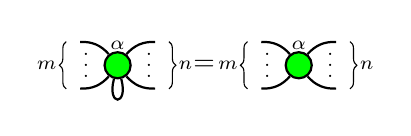
\begin{tikzpicture}
	%
	%
	%
	\begin{scope}[shift={(-0.3,0)}]
	\node [zxgreen,label={[shift={(0,-0.1)}]\scriptsize $\alpha$}] (v0) at (0,0) {};
	\node (v9) at (-0.6,0.3) {};
	\node (v10) at (-0.6,-0.3) {};
	\node (v11) at (0.6,0.3) {};
	\node (v12) at (0.6,-0.3) {};
	\node (d1) at (-0.4,0.1) {\scriptsize $\vdots$};
	\node (d2) at (0.4,0.1) {\scriptsize $\vdots$};
	%
	\draw  (v0) edge[thick,bend right=25] (v9);
	\draw  (v0) edge[thick,bend left=25] (v10);
	\draw  (v0) edge[thick,bend left=25] (v11);
	\draw  (v0) edge[thick,bend right=25] (v12);
	\draw  (v0) edge[thick,loop below, looseness=10] (v0);
	\draw[decoration={brace,mirror,raise=5pt},decorate]
		(v9.east) -- node[left=5pt] {\scriptsize $m$} (v10.east); 
	\draw[decoration={brace,raise=5pt},decorate]
		(v11.west) -- node[right=5pt] {\scriptsize $n$} (v12.west); 
	\end{scope}
	%
	%
	%
	\node at (0.8,0) {$=$};
	%
	%
	%
	\begin{scope}[shift={(1.6,0)}]
	\node [zxgreen,label={[shift={(0,-0.1)}]\scriptsize $\alpha$}] (v1) at (0.4,0) {};
	\node (v9) at (-0.2,0.3) {};
	\node (v10) at (-0.2,-0.3) {};
	\node (v11) at (1,0.3) {};
	\node (v12) at (1,-0.3) {};
	\node (d1) at (0,0.1) {\scriptsize $\vdots$};
	\node (d2) at (0.8,0.1) {\scriptsize $\vdots$};
	%
	\draw  (v1) edge[thick,bend right=25] (v9);
	\draw  (v1) edge[thick,bend left=25] (v10);
	\draw  (v1) edge[thick,bend left=25] (v11);
	\draw  (v1) edge[thick,bend right=25] (v12);
	\draw[decoration={brace,mirror,raise=5pt},decorate]
		(v9.east) -- node[left=5pt] {\scriptsize $m$} (v10.east); 
	\draw[decoration={brace,raise=5pt},decorate]
		(v11.west) -- node[right=5pt] {\scriptsize $n$} (v12.west); 
	\end{scope}
\end{tikzpicture}
\]



\end{document}
